\documentclass[10pt,a4paper]{report}
\usepackage[latin1]{inputenc}
\usepackage{amsmath}
\usepackage{amsfonts}
\usepackage{amssymb}
\usepackage{graphicx}
\usepackage{hyperref}
\usepackage{multicol}
\usepackage[margin=0.5in]{geometry}
\usepackage{tikz}
\usepackage{romannum}
\usepackage{listings}
\usetikzlibrary{arrows,shapes.gates.logic.US,shapes.gates.logic.IEC,calc}
\usepackage{titlesec}
\titlespacing{\subsection}{1pt}{\parskip}{3pt}
\titlespacing{\subsubsection}{0pt}{\parskip}{-\parskip}
\titlespacing{\paragraph}{0pt}{\parskip}{\parskip}
\newcommand{\myvec}[1]{\ensuremath{\begin{pmatrix}#1\end{pmatrix}}}
\let\vec\mathbf

\begin{document}

\centering {
\includegraphics[scale=0.07]{IIT.png}} \vspace{3mm}\\ \raggedleft Name:Somisetty.Kedareswari\vspace{2mm}\\ \raggedleft Roll No.: FWC22049\vspace{2mm}\\ \raggedright Sep 2022 \hspace{12cm} \raggedleft mail2kedari@gmail.com \vspace{10mm}
\\ \centering \Large \textbf{MATRIX ASSIGNMENT} \normalsize \vspace{15mm}
\begin{multicols}{2}
\section{Problem:}  Construct a triangle ABC in which BC=8cm, $\angle{B}=45^0$ and AB - AC = 3.5 cm.\vspace{3mm}
\section{Solution}
The input parameters for this construction are
\begin{center}
\begin{tabular}{|c|c|c|}
  \hline
  \textbf{Symbol}&\textbf{Value}&\textbf{Description}\\
  \hline
  BC & a & where a is 8cm\\
  \hline
  AB & b & AB distance is denoted as c \\
  \hline 
  AC & c & AC distance is deoted as b \\
  \hline
  $\angle{BC}$ & $45^0$ &  $\Delta$ABC \\
  \hline
  $\vec{C}$ & $\myvec{a\\0}$ & BC length is equal to a\\
  \hline
  $\vec{A}$ & $\myvec{ cos\theta \\ sin\theta}$ & using the cosine formula in $\Delta$ABC\\
  \hline
\end{tabular}
\end{center}
\raggedright\textbf{Caluclating Other Coordinate: } \\
\raggedright The coordinates of B and C are $X_{2}$,$Y_{2}$ respectively. \\
  \raggedright Let \textbf{A} =
  $\begin{pmatrix} 
 \cos \theta\\
  \sin\theta \\
\end{pmatrix}$ \\
\raggedright Using the Cosine formula in  $\Delta$ABC, \\ \vspace{3mm}
\begin{equation}
{b}^2\hspace{1.5cm}= {a}^2 + {c}^2 - 2accos\vec{B}
\end{equation}
\begin{equation}
(b+c)(b-c) = {a}^2- 2 \times a \times 0.707c
\end{equation}
Upon Simplifaction we get:- \\
\begin{equation}
  (7-16\sqrt{2})b+7c= -128
\end{equation}
\begin{equation}
        c-b=3.5
\end{equation}\\
     From the above, we obtain the matrix equation:- \\ \vspace{3mm}
        $\begin{pmatrix}
            7-16\sqrt{2} & 7 \\
            -1 & 1  \\
        \end{pmatrix}$% 
        $\begin{pmatrix}
            c \\
            b \\
        \end{pmatrix}$% 
           =
           $\begin{pmatrix}
            -128\\
            3.5\\
        \end{pmatrix}$%   
        \vspace{5mm}           
   \\  
      $\begin{pmatrix}
            c\\
            b\\
        \end{pmatrix}$% 
            =
            $\begin{pmatrix}
            11.99\\
            8.49\\
        \end{pmatrix}$% 
        \vspace{3mm}
   \\  The vertices of $\Delta$ ABC are \\ \vspace{3mm}
     \raggedright \textbf{A} = 11.99$\begin{pmatrix}
                 cos 45 \\ 
                 sin 45 \\
              \end{pmatrix}$%
              =$\begin{pmatrix}
                 8.4 \\
                 8.4 \\
                 \end{pmatrix}$%
                 \vspace{5mm}
              \\ \raggedright  \textbf{B} = $\begin{pmatrix}
                 0\\
                 0\\
              \end{pmatrix}$% 
              \vspace{5mm}
             \\ \raggedright  \textbf{C} = $\begin{pmatrix}
                  8\\
                  0\\
              \end{pmatrix}$%
 \begin{center}
Below python code realizes the above construction : 
\fbox{\parbox{8.5cm}{\url{https://github.com/kedareswari200/fwc-moudle1/blob/Matri_lines/triangle.py}}}
\end{center}
 \section{Construction}
   \begin{center}
  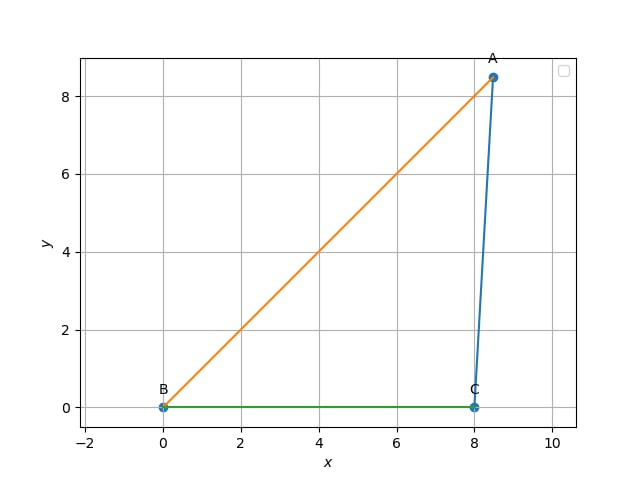
\includegraphics[scale=0.5]{Fig.png}
    \end{center}
\vspace{3cm}
\end{multicols}

\end{document}